% Template for a Computer Science Tripos Part II project dissertation
\documentclass[12pt,a4paper,twoside,openright]{report}
\usepackage[pdfborder={0 0 0}]{hyperref}    % turns references into hyperlinks
\usepackage[margin=25mm]{geometry}  % adjusts page layout
\usepackage[export]{adjustbox}
\usepackage{graphicx}  % allows inclusion of PDF, PNG and JPG images
\usepackage{verbatim}
\usepackage{docmute}   % only needed to allow inclusion of proposal.tex
\usepackage{array}     % for tables
\usepackage{nameref}
\usepackage{rotating}
\usepackage{csquotes}
\usepackage{subcaption}% for subfigures

\graphicspath{ {Images/} }
\raggedbottom                           % try to avoid widows and orphans
\sloppy
\clubpenalty1000%
\widowpenalty1000%

\renewcommand{\baselinestretch}{1.1}    % adjust line spacing to make
                                        % more readable

\begin{document}

%%%%%%%%%%%%%%%%%%%%%%%%%%%%%%%%%%%%%%%%%%%%%%%%%%%%%%%%%%%%%%%%%%%%%%%%
% Title


\pagestyle{empty}

\rightline{\LARGE \textbf{George Andersen}}

\vspace*{60mm}
\begin{center}
\Huge
\textbf{QWOP in JavaScript} \\[5mm]
Computer Science Tripos -- Part II \\[5mm]
Robinson College \\[5mm]
\today  % today's date
\end{center}

\vspace{5mm}


%%%%%%%%%%%%%%%%%%%%%%%%%%%%%%%%%%%%%%%%%%%%%%%%%%%%%%%%%%%%%%%%%%%%%%%%%%%%%%
% Proforma, table of contents and list of figures

\pagestyle{plain}

\chapter*{Proforma}

{\large
\begin{tabular}{ll}
Name:               & \bf George Andersen                       \\
College:            & \bf Robinson College                     \\
Project Title:      & \bf QWOP in JavaScript \\
Examination:        & \bf Computer Science Tripos -- Part II, 2018  \\
Word Count:         & \bf 5300\footnotemark[1]                \\
Supervisor:         & Dr Alastair Beresford                    \\ 
\end{tabular}
}
\footnotetext[1]{Computed using TeXcount http://app.uio.no/ifi/texcount/.

}



\section*{Original Aims of the Project}





\section*{Work Completed}

%All that has been completed appears in this dissertation.

\section*{Special Difficulties}

None.


\section*{Declaration}
I, George Andersen of Robinson College being a candidate for Part II of the Computer Science Tripos, hereby declare that this dissertation and the work described in it are my own work, unaided except as may be specified below, and that the dissertation does not contain material that has already been used to any substantial extent for a comparable purpose.

\bigskip
\leftline{Signed George Andersen}
\medskip
\leftline{Date \today}

\tableofcontents

\listoffigures

%\newpage
%\section*{Acknowledgements}




% %%%%%%%%%%%%%%%%%%%%%%%%%%%%%%%%%%%%%%%%%%%%%%%%%%%%%%%%%%%%%%%%%%%%
% Introduction (intro+prep ~3000)
\chapter{Introduction}

The motivation for this project is to bring together multiple interesting areas of computer science. The project is to recreate an online game called QWOP using JavaScript, and to use a controlled experiment to test how it compares, in the participants view, to the original.
It included implementing a physics simulation, reconstructing the graphics of the game, and investigating the Human Computer Interaction of playing online games.
I decided to use JavaScript for the project as it was a good language for creating an online game, and I was interested in knowing in greater depth how web technologies fit together.
The project would be a challenge as before starting the project I had very limited knowledge of JavaScript, and I would be carrying out a controlled experiment with a large number of participants.
%First of all in this Introduction
In the following section I shall provide an explanation of the game that I have recreated.

\section{What is QWOP?}

QWOP is a browser video game created by Bennett Foddy. The goal of the player is to complete a 100m race without falling over.
Figure \ref{startScreen} shows the screen on game start, which sets the scene for the game and give instructions to the player of how to play. 
% fig of starting screen
\begin{figure}[htbp]
	\centering
	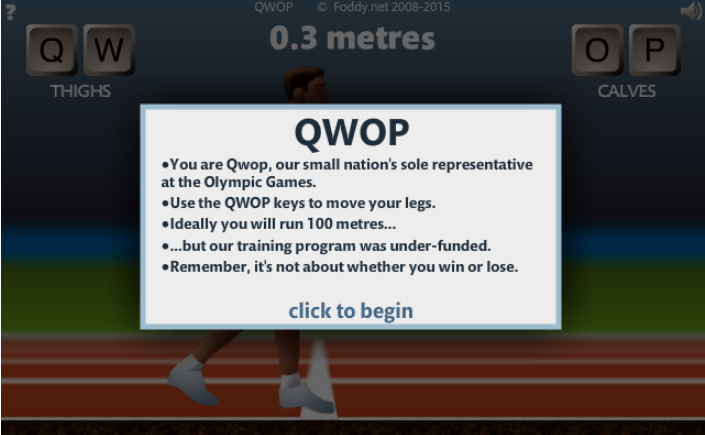
\includegraphics[width=0.6\textwidth]{startScreen.PNG}
	\caption{Starting screen of QWOP}
	\label{startScreen}
\end{figure}


Players control the athlete using only the Q, W, O, and P keys. 
Whilst the Q key is held down, the runner's right thigh is driven forward and his left thigh is driven backward. This moves the legs apart at the bottom of the torso in a scissor-like motion. 
The W key does the opposite of this, and holding it down will put the athlete in a similar stance but with his outstretched legs reversed.
The O and P keys have a similar effect but instead power the movement of the calves. The O key applies a force that moves the left calf towards the back, and the right calf forwards until it is in line with the thigh. Again the P key is the reverse of this.

\begin{figure*}[t!]
    \centering
    % \begin{subfigure}[t]{0.5\textwidth}
    %     \centering
    %     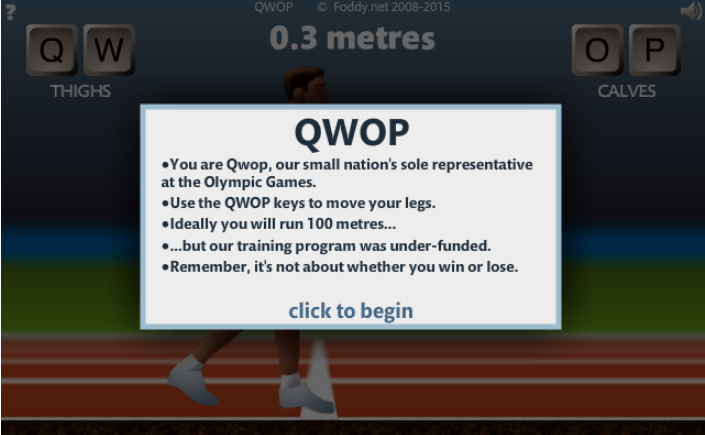
\includegraphics[height=1.6in]{startScreen.PNG}
    %     \caption{Starting screen of QWOP}
    %     \label{startScreen}
    % \end{subfigure}
    \begin{subfigure}[t]{0.45\textwidth}
        \centering
        \includegraphics[height=1.8in]{qwopRunning.PNG}
        \caption{The athlete is running.}
        \label{athleteRunning}
    \end{subfigure}
    ~
    \begin{subfigure}[t]{0.45\textwidth}
        \centering
        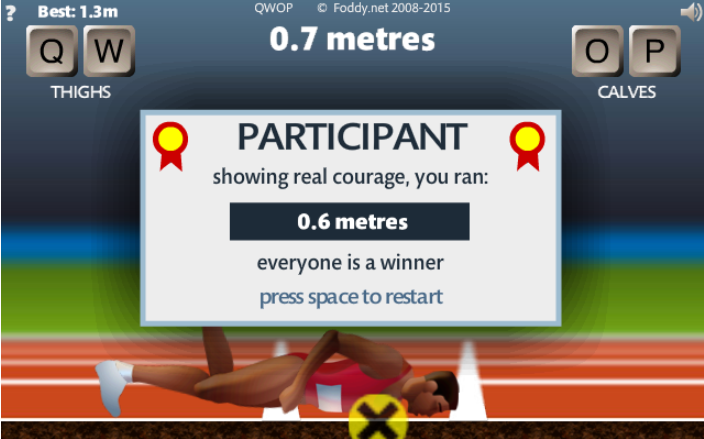
\includegraphics[height=1.8in]{qwopFallen.PNG}
        \caption{The athlete has fallen over so the player must restart.}
        \label{athleteFallen}
    \end{subfigure}
    % \caption{Caption place holder}
    \caption{}
\end{figure*}

Once the player clicks then moves to begin they are free to press the keys to attempt to move forwards. Figure \ref{athleteRunning} shows the athlete running, and this invariably leads to Figure \ref{athleteFallen} which shows the athlete fallen over.
Below the athlete there is an X symbol. This shows where the athlete first touched the floor with his arms or head.
% These section of his body are not allowed to touch the floor as doing so counts as falling over. 
After this the player can press the space bar and start again.
Most players attempt to keep the athlete upright and work out a key combination that will move the athlete in a motion as close to a normal gait as possible.
Others however manoeuvre the runner into a stable position on the floor, and then press lots of keys in the hope that there is some net movement forward.
Both these methods are entertaining and typically lead to some success.
Though the objective of QWOP is simple, it is notorious for being difficult to master ever since it went viral in 2010.



%%%%%%%%%%%%%%%%%%%%%%%%%%%%%%%%%%%%%%%%%%%%%%%%%%%%%%%%%%%%%%%%%%%%
%%%%%%%%%%%%%%%%%%%%%%%%%%%%%%%%%%%%%%%%%%%%%%%%%%%%%%%%%%%%%%%%%%%%
%%%%%%%%%%%%%%%%%%%%%%%%%%%%%%%%%%%%%%%%%%%%%%%%%%%%%%%%%%%%%%%%%%%%
%%%%%%%%%%%%%%%%%%%%%%%%%%%%%%%%%%%%%%%%%%%%%%%%%%%%%%%%%%%%%%%%%%%%
%%%%%%%%%%%%%%%%%%%%%%%%%%%%%%%%%%%%%%%%%%%%%%%%%%%%%%%%%%%%%%%%%%%%
%%%%%%%%%%%%%%%%%%%%%%%%%%%%%%%%%%%%%%%%%%%%%%%%%%%%%%%%%%%%%%%%%%%%
% Preparation (intro+prep ~3000)
\chapter{Preparation}

In this chapter I will discuss the preparation that happened before the implementation of the project began.
In section \ref{mathModel} a mathematical model of QWOP is developed that is built in the implementation chapter.
% Starting point?
As suggested in the Project Proposal, I used Phaser to create my JavaScript version of QWOP. One of the first things that I did to prepare was to learn how Phaser works. In section \ref{phaser} I shall give a brief description of what Phaser is and how it works.
Section \ref{stats} goes through the statistical tests that we're learned before the analysis in the evaluation could take place.


\section{Mathematical model of the QWOP world}
\label{mathModel}
% Model needed explanation
To create QWOP in a physics simulation it first helps to know how it is going to be modelled. So when preparing it was important to first design a mathematical model of the QWOP world that could later be implemented in a physics simulation.
%\subsection{Planar rigid-body mechanics}
%\label{planar}
The basis of this model is planar rigid-body dynamics.
% https://en.wikipedia.org/wiki/Rigid_body_dynamics
As the floor that the athlete is standing on and the limbs of the athlete do not change size and do not need to deform, they can be modelled as rigid bodies.
Save the floor, each of these rigid bodies represent one section of the athlete that has it's own position and rotation. For example the foot, upper leg and lower leg.
%should insert some rbd formulas somewhere here?
Planar rigid-body mechanics uses kinematics, and solves the equations of motion described by Newton's second law to determine the motion of the bodies in the system.
%The acceleration, velocity and position of the rigid bodies can be determined using kinematics, and by solving the equations of motion described by Newton's second law.
Since this model can describe the acceleration, velocity and position of the individual rigid bodies over time, the system as a whole under the effects of gravity can be simulated.
% Finish this next
With only basic planar rigid-body dynamics, the limbs will simply fall to the floor. So next I will describe the required extensions to this model that emulate the behaviour of QWOP.

\subsection{Joints}
\label{sub:joints}

% Joints explanation
The members of an athlete are connected by joints. For example the foot and lower leg are connected at the ankle, and the lower leg and upper leg are connected at the knee.
%This is a constraint that the joints force the members to follow.
These constraints need to be captured in the model.
For each joint-body connection, the joint stays in the same position relative to the frame of reference of the body -- joints maintain a consistent offset from each connected member. For example, the ankle is always at the back of the foot, and the ankle is always at the bottom of the lower leg. These two constraints work together in each joint to connect two limbs.
In the same way, the mathematical model of QWOP will include joints that enforce these constraints.
% Angle limiting explanation
Another function of an athlete's joints is to limit the angles the limbs can rotate. For example the knee allows the lower leg to rotate up until the point where the upper and lower legs are in a straight line. In the same way the joints in the model limit the angle each rigid body can rotate.

\subsection{Collisions}
\label{sub:collisions}
% Collision boxes
A final constraint the limbs follow is that they collide with the floor.
Each rigid body has an area, and the areas of the limbs and the area of the floor cannot overlap, otherwise the athlete would fall through the floor.
For this reason the model needs to take collisions between the limbs and floor into account.
To model this each rigid body can have a rectangular collision box, specified by a width and height.
The boxes for the limbs can then be stopped from entering the box representing the floor.s
The collisions between the limbs do not however need to be taken into account, as one limb can go behind another in the 2D view the user can see.

\subsection{Forces}
\label{sub:forces}
% So far rigid bodies and joints
The QWOP world so far amounts to a set of rigid bodies and a set of joints on which the physics of planar rigid-body dynamics can be applied.
There are 13 rigid bodies in total; firstly a foot, lower leg, upper leg, lower arm and upper arm for each side of the body, and also a torso, head and finally the floor. Each of these have a width and height that define their collision box, a starting position, and a mass.
The values of these variables are such that the floor is immoveable and spans the bottom of the world, and the attributes of the rigid bodies match the attributes of the limbs of the QWOP athlete.
There are 11 joints in total; a left and right ankle, knee, hip, shoulder, elbow, and a single neck. Each of these specify which two rigid bodies they join together, the offset from each of those bodies that the joint must stay, and the maximum and minimum angles between which the joints can rotate. These connect the limbs together in the right order and keep them together with the physical properties of an athlete.

This model so far delivers an athlete with limbs that can move in Cartesian space whilst checking for collisions with the floor, and rotate freely whilst keeping joint constraints.
A final addition to the model is a method of applying forces to the rigid bodies just as the muscles of an athlete would apply forces to its limbs.
These include two types of forces, firstly the force when actively driving a limb forward. Secondly the forces that I will call static rotational forces. These static forces keep the body in the same shape when a limb is not being actively driven forward.
For example if the player is not pressing any keys, then the athlete should hold his shape and start falling in whichever direction is natural, rather than collapsing to the floor.


\section{Understanding Phaser}
\label{phaser}

Phaser is a Desktop and mobile HTML5 game framework that is designed to take care of the mundane tasks involved with developing a game so that development can be sped up. It helps the developer focus on the creative aspect of game design as time is not wasted on reinventing the wheel.

Phaser handles jobs such as creating the canvas the game will be drawn to, and provides frameworks that handle compatibility issues. For example it provides access to simple methods for drawing graphics onto the canvas, and responding to user input, whether on a mobile device with a touch screen, or on a desktop with a keyboard and mouse.
%It also organises execution flow around the program and

To take advantage of these features, a developer first imports the Phaser library by adding the minified script to their web page. %using this html code:


\begin{displayquote}
	\texttt{<script type="text/javascript" src="js/phaser.min.js"></script>}
\end{displayquote}

It is then possible to start off ones JavaScript code with a line similar to this:

\begin{displayquote}
	\texttt{var game = new Phaser.Game(gameWidth, gameHeight, Phaser.CANVAS, 'game-name', { preload: preloadFunction, create: createFunction, update: updateFunction, render: renderFunction});}
\end{displayquote}

This code shows how the Game object is created.
% I shall explain this code as it explains Phaser.
The Game object is the main controller for the entire Phaser game. 
First of all it handles the boot process. The boot process creates the canvas dimensioned to the width and height parameters provided and initialises Objects and data structures that will be used later.
After it has initialised the game, the event-based paradigm is used to pass control flow to code the developer has written. 
This simplifies controlling the execution flow
%over the lifetime of the game 
by giving the developer access to execute code at key moments in execution called events.
This is helpful as the developer doesn't have to write a lot of boilerplate code to organise this themselves.
When one of these events arise, a callback function that the developer has written is executed. In argument four of the above code, the developer passes a JavaScript object to specify the callback functions for each event.
One of the object's named argument pairs is \texttt{update:updateFunction}, so here the developer has given the identifier \texttt{updateFunction} to be used for Phaser's \texttt{update} operation. This means that the contents of updateFunction will be run once every frame.
In a similar way the developer can write a \texttt{preload} function that loads assets before the game starts that Phaser will run at the beginning of the game.

\subsection{Sprites}
\label{sprites}

Another feature of Phaser is its use of sprites.
In the Phaser documentation \footnote{definition from https://photonstorm.github.io/phaser-ce/Phaser.Sprite.html}
sprites are described like so:

\begin{displayquote}
``At its most basic a Sprite consists of a set of coordinates and a texture that is rendered to the canvas. They also contain additional properties allowing for physics motion (via Sprite.body), input handling (via Sprite.input), events (via Sprite.events), animation (via Sprite.animations), camera culling and more.''
\end{displayquote}

These are multi-purpose objects that are used to add components to a game. At base they are a set of $x$-$y$ coordinates and a texture. For example to add a character to the game, one can choose an image to use as a texture, which can then be moved around the canvas by changing the coordinates of the sprite.
Extra functionalities can be added to make use of other parts of Phaser, such as adding functions that handle certain inputs to the game, or adding animations.

todo: finish this

\subsection{Physics engines}
Phaser also comes with three different options of physics engines, ``Arcade'', ``Ninja'' and ``P2''. The difference between these options is that they start off simple and increase in complexity. This is useful as lightweight engines are preferred if the game is going to but run on a low-powered device such as a mobile phone. P2 is the most complex and has support for full body systems, including springs and collisions.


\section{Statistical tests}
\label{stats}
% https://www.graphpad.com/support/faqid/1790/
To prepare for the evaluation chapter I investigated some statistical tests. 
Since lots of data is collected in the evaluation, statistical tests needed to be compared to find appropriate ways of comparing this data, for example comparing the distances participants reach over the two games.
In this example a parametric test such as a t-test would be inappropriate, since the participants are trying to go forwards the distances reached will likely not be from a Gaussian or another symmetrical distribution.

The Kolmogorov–Smirnov test would be more useful in this case, as it gives a distance between. The data does not need to be paired as 

since data will likely not be paired, 

todo: keep writing this - add other ideas used in eval and how prepped


% Next I learnt how to do these thingys
% stuff in course
% 	stats test
% 	open coding?

In this chapter, I have discussed the theory that had to be understood, and work that
had to be done, before implementation could begin.




%%%%%%%%%%%%%%%%%%%%%%%%%%%%%%%%%%%%%%%%%%%%%%%%%%%%%%%%%%%%%%%%%%%%
%%%%%%%%%%%%%%%%%%%%%%%%%%%%%%%%%%%%%%%%%%%%%%%%%%%%%%%%%%%%%%%%%%%%
%%%%%%%%%%%%%%%%%%%%%%%%%%%%%%%%%%%%%%%%%%%%%%%%%%%%%%%%%%%%%%%%%%%%
%%%%%%%%%%%%%%%%%%%%%%%%%%%%%%%%%%%%%%%%%%%%%%%%%%%%%%%%%%%%%%%%%%%%
%%%%%%%%%%%%%%%%%%%%%%%%%%%%%%%%%%%%%%%%%%%%%%%%%%%%%%%%%%%%%%%%%%%%
%%%%%%%%%%%%%%%%%%%%%%%%%%%%%%%%%%%%%%%%%%%%%%%%%%%%%%%%%%%%%%%%%%%%
%%%%%%%%%%%%%%%%%%%%%%%%%%%%%%%%%%%%%%%%%%%%%%%%%%%%%%%%%%%%%%%%%%%%
%%%%%%%%%%%%%%%%%%%%%%%%%%%%%%%%%%%%%%%%%%%%%%%%%%%%%%%%%%%%%%%%%%%%
%%%%%%%%%%%%%%%%%%%%%%%%%%%%%%%%%%%%%%%%%%%%%%%%%%%%%%%%%%%%%%%%%%%%
%%%%%%%%%%%%%%%%%%%%%%%%%%%%%%%%%%%%%%%%%%%%%%%%%%%%%%%%%%%%%%%%%%%%
% Implementation ~4500
\chapter{Implementation}
This section details the implementation of the mathematical model of QWOP 
designed in Section \ref{mathModel}, and the implementation of the evaluation scaffolding used during the user study.
Section \ref{sec:qwopImp} focuses on the implementation of QWOP
(need to add what other subsections do).
Section \ref{studyimpl} explains the code written to produce and analyse the results of the user study.
(again add subsections of this once done) 

% This chapter describes the implementation of the project, moving on from preparation in previous chapters. The main implementation tasks in the project were writing my version of QWOP, and writing the set of software used to perform the user study and evaluate the project. These can be divided as follows:

\section{Phaser Implementation of QWOP}
\label{sec:qwopImp}
As in the project proposal, I have used Phaser to implement my version of QWOP in JavaScript.
I provided an overview of what Phaser is and how it works in Section \ref{phaser}.
I will now describe how it was used to make the different components of the game. First I shall show how it implemented the mathematical model of QWOP described in Section \ref{mathModel}.

\subsection{Modelling the athlete}
\label{sec:athleteModel}
The first task of my code is to create the model of the athlete, that is later built into the physics system. This starts with declaring the variables describing all the dimensions of the model.
These variables lay out the dimensions of each limb, including their height, width, mass and starting rotation. They also specify the properties of the joints, for example the maximum and minimum angle that the joints can rotate to. Finally other values set forth other aspects of the model, such as the offset of the head from the top of the torso, or the distance between the left and right shoulder. 
These values specify the model of the athlete.
% all adapted to be like an athlete.

After these variables have been defined, a second set of variables are derived from them that will be used later. To do this forward kinematics is used on the previous set of variables to work out the starting coordinates of each limb. The code takes the starting position of the torso, and then uses the height of the torso and other offsets to get the $x$ and $y$ values for where the left upper arm should start. Then it uses the starting rotation, width and height of the upper arm to work out the starting position of the lower arm. This is repeated over all the limbs, until the $x$ and $y$ values of the starting positions are specified for all of the rigid bodies.

%To model the athlete from these sprite joints, I specified the dimensions, mass, offset and starting rotation of each limb. Then
%The limbs are then instantiated in these starting positions with the correct mass, dimensions and 'revoluteConstraint' joints. 



\subsection{Planar Rigid-Body Mechanics}
Now that the model of the athlete has been defined, the core of the mathematical model, planar rigid-body mechanics, is implemented. To implement the Planar rigid-body mechanics of Section \ref{mathModel}, I used P2, one of the physics engines that comes with Phaser.
P2 and other aspects of Phaser such as the game object have been described in Section \ref{phaser}.
The next section of my code first runs the set-up described there, after which the P2 physics system is initialised with this code:

\begin{displayquote}
	\texttt{game.physics.startSystem(Phaser.Physics.P2JS);}	
\end{displayquote}

P2 uses sprites, as I described earlier in section \ref{sprites}. One of their functionalities is that they can be added to one of Phaser's physics systems, meaning that their $x$ and $y$ values are controlled to follow the physics rules you set up.
In this code, a sprite is created and added to the game object.

\begin{displayquote}
	\texttt{head = game.add.sprite(headX , headY , 'head');}
\end{displayquote}

The \texttt{headX} and \texttt{headY} values in the above code are the $x$ and $y$ values of the head defined earlier. Similar code is repeated over all of the $x$ and $y$ variables to create a sprite for each rigid body of the model.

These sprites are then enabled in the physics system using this code:

\begin{displayquote}
    \begin{verbatim}
	game.physics.p2.enable([torso, upperLegLeft, lowerLegLeft, shoeLeft,
      upperLegRight, lowerLegRight, shoeRight, upperArmLeft,
      lowerArmLeft, upperArmRight, lowerArmRight, head, floor],false);
    \end{verbatim}
\end{displayquote}

This allows P2 to control their coordinates.


\subsection{Modelling joints in physics}
\label{sec:jointsInPhysics}

Figure \ref{swingingRods} shows my first prototype for modelling joints and limbs. The rods are held together by joints and can swing freely. Each rod is a sprite, and each joint connecting them is the joint used to control rotations in P2 physics, called a \texttt{revoluteContraint}.

\begin{figure}[tbh]
\centerline{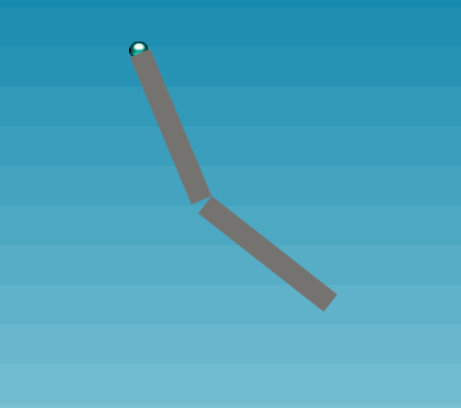
\includegraphics[scale=0.5]{swingingRods.PNG}}
\caption{Swinging rods initial model of limbs}
\label{swingingRods}
\end{figure}

The next stage of my code implements section \ref{sub:joints} of the mathematical model, the joints between the rigid bodies.
These joints are created between the sprites created earlier. The code below implements the left ankle, the joint connecting the left foot with the left lower leg:

\begin{displayquote}
	\begin{verbatim}
    ankleLeft = game.physics.p2.createRevoluteConstraint(shoeLeft,
        [-shoeXOffset,-shoeLegDistance],lowerLegLeft,
        [0,lowerLegHeight/2],maxForce);

    ankleLeft.upperLimit = ankleMaxAngle;
    ankleLeft.lowerLimit = ankleMinAngle;
    \end{verbatim}	
\end{displayquote}

Firstly the \texttt{RevoluteConstraint} joint is created. The first and third arguments specify the sprites in the physics system that are to be connected together by the joint. In this case the left foot sprite is connected to the left lower leg sprite. The second and fourth arguments set the offset from the centre of each limb that the joint should stay. Here the ankle should always be at the top and towards the back of the foot, and it should be at the bottom of the lower leg, \texttt{lowerLegHeight/2} from the center of the lower leg.

Secondly the upper and lower limits of the ankle are set to stop the ankle rotating into impossible positions. Again the angle variables used are the variables that specified the model earlier, and similar code is repeated for all the joints in the model.

%%%%%%%%%%%%%%%%%%%%%%%%%%%%%%%%%%%%%%%%%%%%%%%%%%%%%%%%%%%%%%%%%%%
% Older versions

% https://cdn.rawgit.com/gla23/Part2Project/b43f453d1597b3f8080149ee5ca01760d64828dc/QWOPjs.html
% swinging rods

% https://cdn.rawgit.com/gla23/Part2Project/2b6292ed7cc0cb4994fea7af4697a1c1091b484d/QWOPjs.html
% 1 leg 

% https://cdn.rawgit.com/gla23/Part2Project/90935e3f9d1c2ff3d96cb271449743c98e651588/QWOPjs.html
% body without graphics

%https://cdn.rawgit.com/gla23/Part2Project/a76f298dcf66717188357c85e1b0b7667cea8e46/myQWOPjs.html
% with graphics


\subsection{Applying the joint forces}
\label{sec:powerInPhysics}


In Section \ref{sub:forces}, the mathematical model of QWOP describes two types of forces used by the athlete. Firstly active forces that the athlete uses to drive a limb forward, and secondly static rotational forces that are used to keep the body in shape so that it does not collapse to the floor.
In the previous section of code, the joints are created, and now they are used to implements these forces.
The mechanism used to apply these forces is to use a set of methods build into Phaser's \texttt{RevoluteConstraint} object that add the functionality of a motor to the joint.
The motor applies a force over its two sprites such that the angular velocity of the joint will increase or decrease towards the motor speed. This force it applies is limited by the maximum torque of the motor, which is set by the \texttt{motorMaxTorque} variable belonging to each \texttt{RevoluteConstraint} joint.
The motor is turned on and off with \texttt{enableMotor()} and \texttt{disableMotor()}, and the speed set with \texttt{setMotorSpeed()}. Both types of forces are applied using the same method, as if the Motor speed is set to a positive value, the motor will increase the angular velocity to that value, which drives the limbs forward. Whereas if the motor speed is set to 0, the motor will apply the necessary forces to stop the joints from rotating so that the athlete stays in shape. 
%The \texttt{motorMaxTorque} value again limits the up to the maximum torque.

%todo: how inputs are connected to the motors

%todo: collision boxes

%The motors for these joints are then attached to the user input according to the control scheme. If a key is pressed that powers the limb, the motor is set to the limb power, otherwise it is set to 0 so that the passive forces apply.



\begin{figure}[tbh]
\centerline{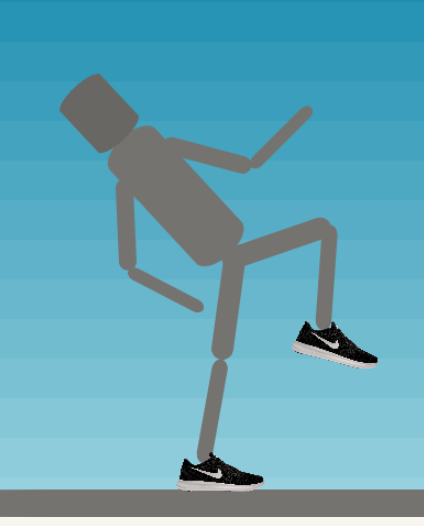
\includegraphics[scale=0.5]{athleteModel.PNG}}
\caption{Model of athlete}
\label{athleteModel}
\end{figure}

\subsection{Graphics}
\label{sec:graphics}

Once I had implemented the mathematical model of QWOP in the physics simulation, the next stage was to change the graphics so that it looked similar to the original QWOP.
To do this, I used the Chrome developer tools to access the files that the original QWOP downloaded when loading. In these files I found an image containing the graphics for the athlete, and other images for other components such as the background and help screens.
To add these graphics into the game, I separated the textures into separate images, and set them as the textures for the corresponding sprites.
Figure \ref{modelWithGraphics} shows the implementation of the model after the graphics had been added.

\subsection{Game flow}
\label{sec:gameFlow}
After the core components of the game were implemented, I added the other components needed to emulate the original QWOP.
Firstly, calculating the distance the player has run so far. To do this I wrote a function that took the $x$ value belonging to the athletes torso in the physics simulation, and returned a distance in meters. The function calculates the distance between the athlete and the starting line, and scales it such that 
it is the same distance the original judges you to have reached, for moving the same distance along the screen.

\begin{figure}[tbh]
\centerline{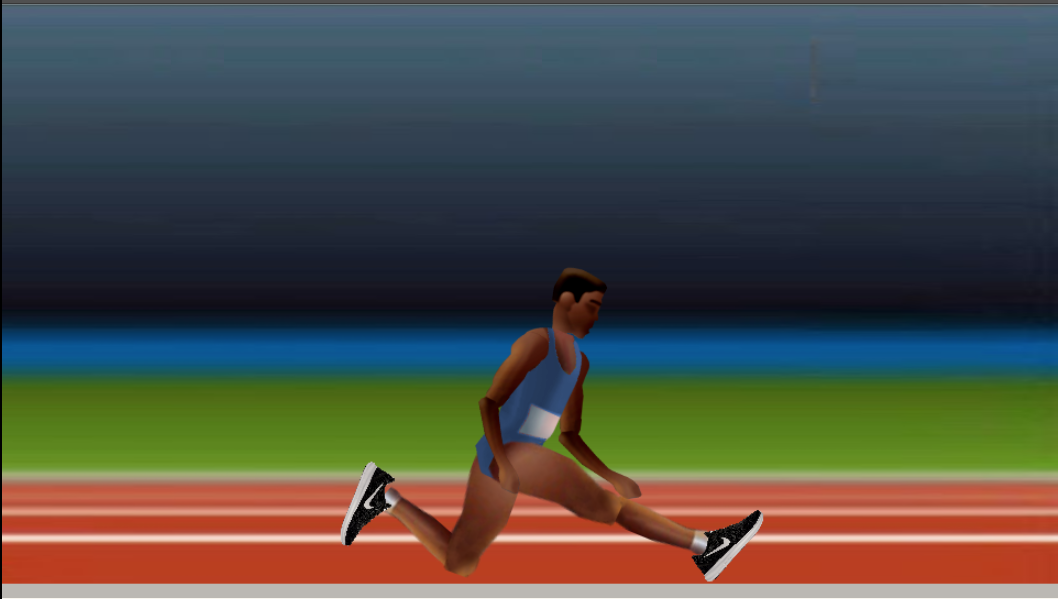
\includegraphics[scale=0.4]{Images/modelWithGraphics.PNG}}
\caption{Model with graphics added}
\label{modelWithGraphics}
\end{figure}

Other components added include the text which updates to show the distance the athlete has reached, the ability to record a high-score the user had got, and text to display the current high-score on the screen.
The text that shows how far you have reached updates ever frame, and is changed in the 
\texttt{update} function.
The way Phaser controls execution flow using callback functions such as \texttt{update} is described in Section \ref{phaser}.
Here is an excerpt of the \texttt{update} function showing the text being updated each frame of the game:

\begin{displayquote}
	\begin{verbatim}// Update Score Text
currentScore = distanceTraveled();
scoreText.text = currentScore + " meters";
// Check if the player has won the game
if (gameOver == false && currentScore>100) {
    gameOver = true;
    coverSprite = game.add.image(gameWidth/2,gameHeight/2, 'gameWon');
}\end{verbatim}
\end{displayquote}

The second function of this code is to check whether the athlete has reached the end of the 100m. If so it displays the congratulations message and allows the player to restart. The Final components I added were the help boxes that are shown when the game begins, when the athlete falls over, and when the game has been completed as in the code above.


\begin{figure}[tbh]
\centerline{\includegraphics[scale=0.8]{userStudyFlow.pdf}}
\caption{Diagram of user study flow}
\label{flow}
\end{figure}

\section{Implementation of evaluation software}
\label{studyimpl}

To evaluate the project, I will be analysing the results from the user study. 
The evaluation chapter contains this analysis, however a large amount of work went into implementing the testing environment, so I will describe that here.
Figure \ref{flow} shows the sections of the study.

First of all the participants are briefed on what the study will contain, and are informed of their ability to opt out whenever they wish. If a participant decides to opt out, their data will be deleted.
After participants have given their informed consent to take part in the study, they move on to the rest of the study, which is hosted on a webpage. The first section asks the user to fill in a Google form.
This first questionnaire finds out the demographics and previous experience of each participant. 
The main component of the study follows.
In a controlled experiment, each participant is randomly placed into one of two groups. The two groups play both versions of QWOP in a different order.
Each game is instrumented, so that while the participants play, their key presses and the distance reached down the track are recorded. Both versions are played for 5 minutes before the study moves onto the next section.
After the users have used the instrumented software, they fill out a second questionnaire that records the opinions of the participant through questions such as 
``Which version felt like you had more control over the athlete?'' and
``Why do you think this was?''.

The Evaluation chapter goes into detail explaining the design choices for the user study, and analyses its results. In the next section I will explain the implementation of the code and the other elements of the evaluation scaffolding used to facilitate the user study.



\subsection{Implementation of the webpage hosting the user study}
\label{sec:webpage}

To host the user study, I wrote a webpage that guides the users through the sections of the study, shown in Figure \ref{flow}.
The webpage consists of an HTML page and JavaScript file that controls the use of the page.
The HTML page contains elements for the page title, multiple elements for text, a \texttt{Next} button, and an iframe that hosts another website.
The button is used to move to the next section of the study. When clicked, the contents of the other elements are updated to construct the next section of the study. The text gives instructions for how the participants should continue, and the iframe contains one of the questionnaires or one of the instrumented versions of QWOP.

Hosting the study on the webpage allowed participants to take part in my user study concurrently, which helped me maximise the number of people taking part in the study.
Other benefits of hosting the user study on a webpage were that it was simple to embed Google form questionnaires, and I could host instrumented adaptations of both versions of QWOP to log data from the experiment.

\begin{figure}[tbh]
\centerline{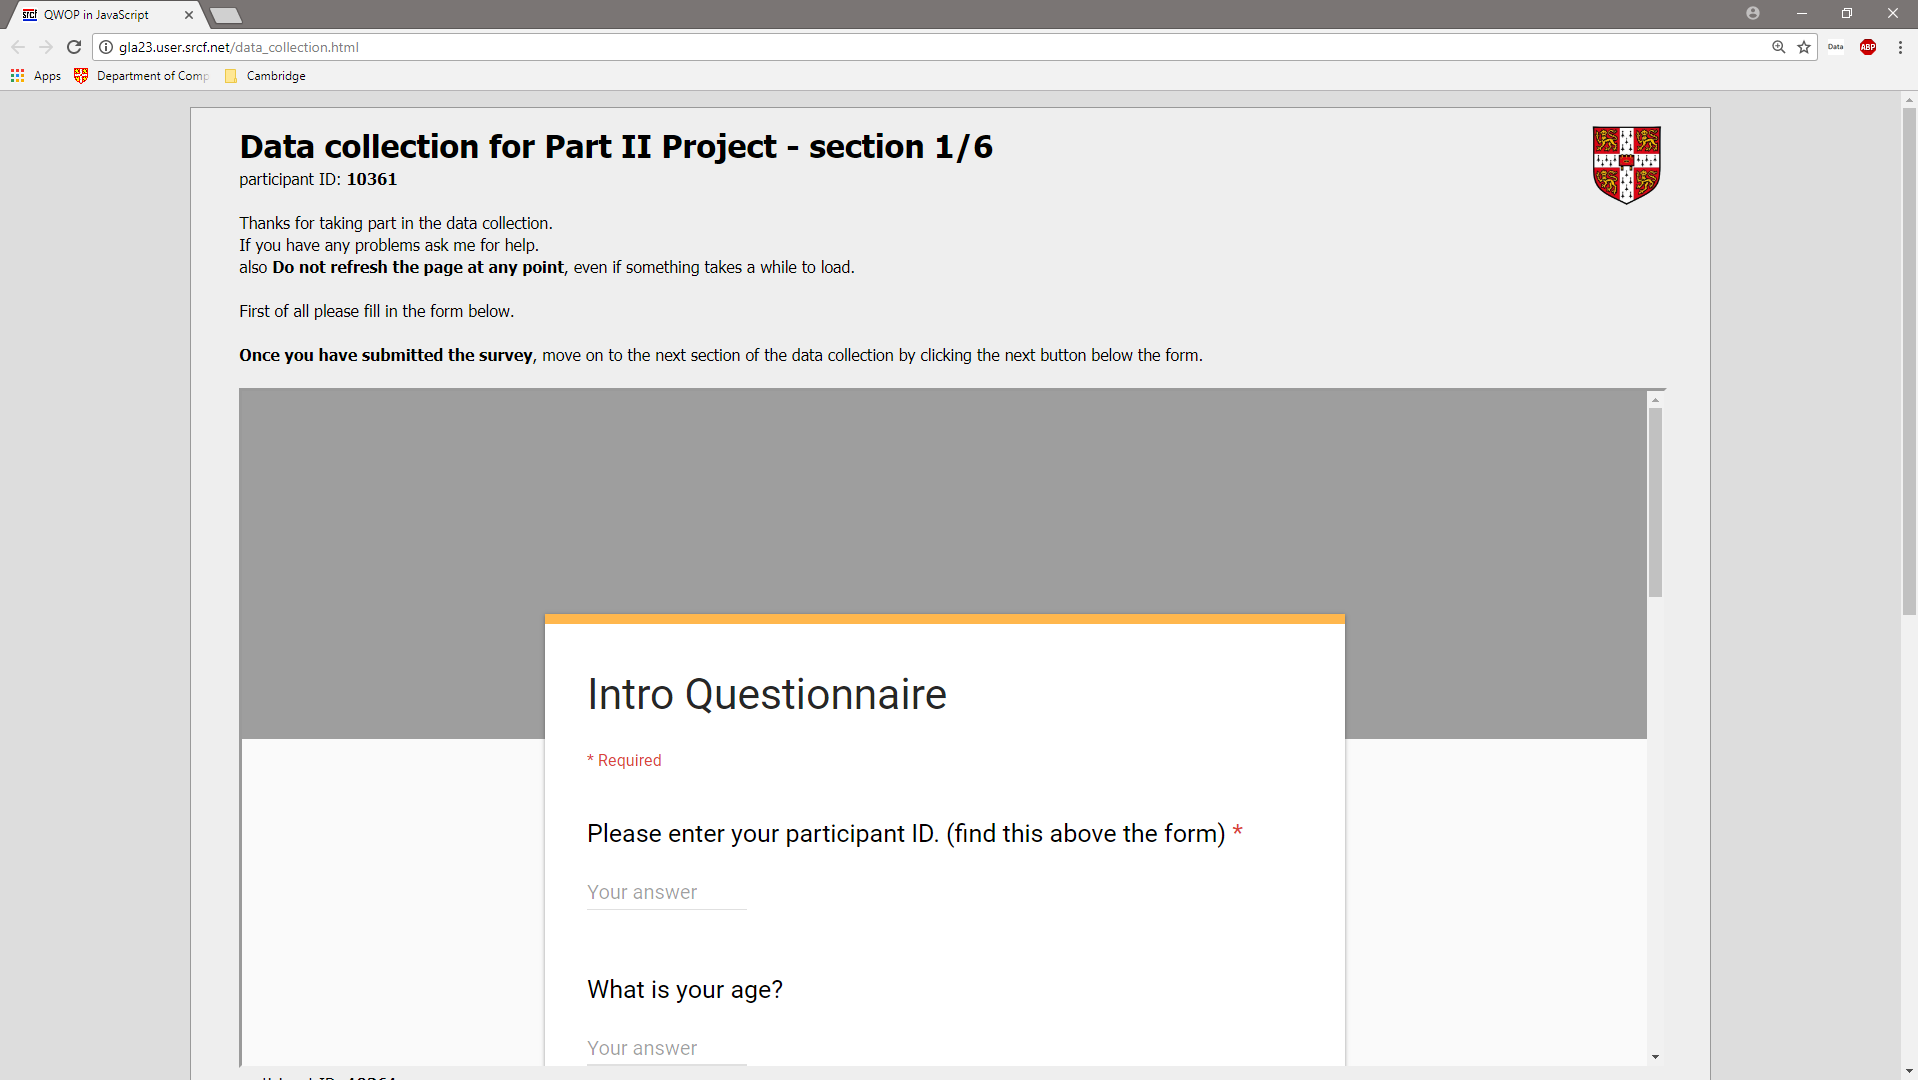
\includegraphics[scale=0.54]{userStudyWebPage.PNG}}
\caption{Opening page of the user study}
\label{study1}
\end{figure}

I hosted the web page on my SRCF web space. Whilst the web page is recording data, it logs the data by sending it to the server at regular time intervals.
I wrote a PHP script that the server uses to process this data server-side and record it into separate files for each participant. This creates a JSON database of all the key-presses and distances travelled for the participants, which means that a group of participants can take part in the study, and then afterwards all the data is easily accessible server-side.

\subsection{Chrome extension for reading distance from QWOP}
\label{sec:chromeExtension}

% todo: Start by telling me what the problem is.  Is it that the implementation didn't expose its distance variable to something else? You see I don't understand -- and it's your job to help me feel I do understand your program, and this needs you explaining in more detail :-)
%todo: redo with alan's comments

Later on in the implementation I encountered a problem when instrumenting the original QWOP. I discovered that I couldn't access the distance that the player had run down the track.
To host the original on my data collection page, the website for the original was placed in the iframe. This let the user play the game, although it was impossible for my page to access any internal data from the outside, since all the game data is inside an anonymous function.

To instrument my version I added code to log the key-presses and send the key log buffer and current distance to the server at regular intervals. I inserted similar code into the iframe of the original to record key-presses, however since the internal data of the game was not accessible, I had to find another method of accessing the distance the player had reached.

Another method I attempted
% to try and access the distance
was to take the HTML, JavaScript and other local resources that the game accessed, and run them locally. In this way an edited version could be run that outputs the distance travelled.
This did not work as the game appears to run some counter hosting measures such that the game does not start, and instead, the canvas goes orange.
Since this did not work I tried accessing the colour values of the game's canvas, so that I could use OCR to read the distance from the screen itself. This did not work however as accessing the pixel values from the canvas inside the iframe was blocked. The original QWOP has a OpenGL setting that made the GLBuffer unreadable.
In the end I solved this problem by creating a chrome extension that took a screenshot of the page over regular intervals so that OCR could be used.
The extension used it's developer privileges to take a screenshot of the page and place it in a canvas. The data collection page then locates the text in the screenshot that shows how far the player has run, and uses a lightweight JavaScript OCR script called ocrad.js
\footnote{ocrad.js is available at http://antimatter15.com/ocrad.js/demo.html} to read the distance the athlete has travelled.
The script gave accurate results with a some editing of the output after the colours of the input image are inverted so that it's black text on a white background.

% Something about I learnt how to do extension marks pls
% todo summary of impl

%%%%%%%%%%%%%%%%%%%%%%%%%%%%%%%%%%%%%%%%%%%%%%%%%%%%%%%%%%%%%%%%%%%%
%%%%%%%%%%%%%%%%%%%%%%%%%%%%%%%%%%%%%%%%%%%%%%%%%%%%%%%%%%%%%%%%%%%%
%%%%%%%%%%%%%%%%%%%%%%%%%%%%%%%%%%%%%%%%%%%%%%%%%%%%%%%%%%%%%%%%%%%%
%%%%%%%%%%%%%%%%%%%%%%%%%%%%%%%%%%%%%%%%%%%%%%%%%%%%%%%%%%%%%%%%%%%%
%%%%%%%%%%%%%%%%%%%%%%%%%%%%%%%%%%%%%%%%%%%%%%%%%%%%%%%%%%%%%%%%%%%%
%%%%%%%%%%%%%%%%%%%%%%%%%%%%%%%%%%%%%%%%%%%%%%%%%%%%%%%%%%%%%%%%%%%%
% Evaluation (eval+conc ~ 2500)
\chapter{Evaluation}
\section{Success Criteria}

%In my project proposal the success criteria is defined like so:
Referring back to the project proposal,
I proposed to evaluate the project with a user study:
%sthe aims of the project are described like so:

\begin{displayquote}
``At the end of the project I expect to be able to demonstrate a game similar to that of the original QWOP.
% [...] although I am not aiming to replicate the behaviour of the original QWOP exactly [...]
%/\end{displayquote}
%\begin{displayquote}
% The athlete should have the same physical qualities that make it seem human, and the game should have the same gameplay items that make it work. The Work to be done section breaks down how this will be done in more detail.
I propose to test how successful the project is with a user study. Since the quality of a game is subjective, it is appropriate to do a user study...''
\end{displayquote}

%I shall now clarify these objectives of the project into some success criteria.
In order to test the success of the project, I refined the success criteria.
The rest of the evaluation, including the user study will provide evidence that these criteria have been met.
The success criteria are:

\begin{enumerate} 
	\item I have developed a game similar to that of the original QWOP in JavaScript.
	\item My version is faithful to the original QWOP; it contains the same mechanics 
    and provides a similar playing experience.
	% \item My version will be different in some aspects, to the improvement of the game. Since measuring `improvement' is subjective, a metric I can use is the enjoyment of the game for a typical player.
    \item My version aims to be more playable for a typical player and I will quantify the improvement in a user study.
\end{enumerate}

% the stats show that it is similar
% i made some changes to make it easier and more fun for players
% new curve
Previously, the Implementation chapter described the components of the user study. Figure \ref{flow2} shows how a participant progresses through these sections.
Section \ref{studyimpl} of the implementation chapter explains the implementation of the system used to facilitate the user study, including the code written for the webpage, and how the games were instrumented.
The rest of this chapter will explain the design choices for the user study, and analyse its results.

\begin{figure}[tbh]
\centerline{\includegraphics[scale=0.8]{userStudyFlow.pdf}}
\caption{Diagram of user study flow}
\label{flow2}
\end{figure}

After participants have given their informed consent to take part in the study, they move on to the first questionnaire, which is hosted on the data collection webpage. 
In section \ref{q1} the results of this first questionnaire are analysed.

The main component of the study follows, the controlled experiment.
In Section \ref{expResults}, the controlled assessment will be explained, and the data recorded during the controlled experiment will be presented and analysed.

After the users have used the instrumented software, they fill out a second questionnaire that records the opinions participants have of the two versions. The results of this questionnaire are given in section \ref{q2}.


\section{Intro Questionnaire Responses}
\label{q1}

The participants that took part in the study were students, some of whom I recruited at the Computer Laboratory. I set up the user study software on a few computers in the Intel Laboratory and recruited people in person and through social media.
The first questionnaire asked for the demographics of each participant.
% 30 participants took part in the user study. This is a good number because...
Figure \ref{demographics} shows the age and gender of the 30 participants that took part in the study.

\begin{figure}[tbh]
\centerline{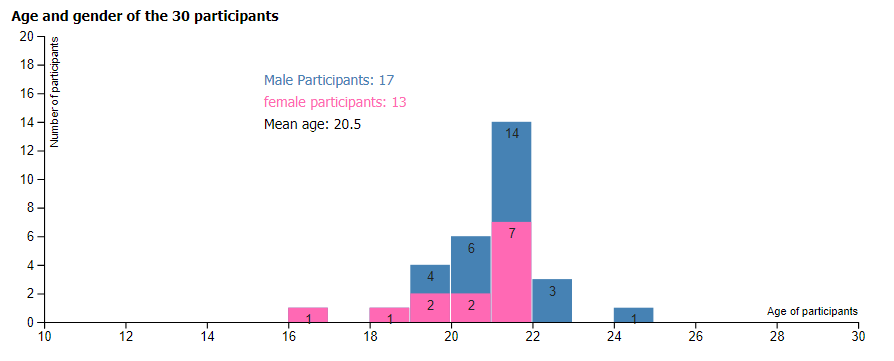
\includegraphics[scale=0.7]{participantDemographics.pdf}}
\caption{Participant demographics}
\label{demographics}
\end{figure}

In order for my controlled experiment to have good external validity, it was important that the recruited participants were representative of the population for which I want to make conclusions.
According to a study by the Pew Research Center\footnote{http://www.pewinternet.org/2008/12/07/adults-and-video-games/} younger people and students are more likely to play games than others:

\begin{displayquote}
``Independent of all other factors, younger adults are considerably more likely than older adults to play games, and the likelihood that an adult is a video gamer decreases significantly with age.

A person's education level is another predictor of video game play. Some 57\% of respondents with at least some college education play games, significantly more than high school graduates (51\%) and those who have less than a high school education (40\%). Current students who are 18 or older are also avid players.''
\end{displayquote}

The Evaluation Criteria show that the study aims to make conclusions about a typical QWOP player.
Since the recruited participants were younger people and students, they represent a typical game player and hence QWOP user. So in this regard the study has good external validity.

% Design considerations:
% Reliability (Would you get the same measurement again?)
% Validity (Are you measuring what you claim to be measuring?)
% Internal validity is the relationship between your measurement and what you think it tells you about the experimental task.
% External validity is the relationship between what you measure in the lab, and the phenomenon in the outside world.


The next question of the questionnaire asked whether the user had played QWOP beforehand. Figure \ref{previousExperienceTable} shows the options that were available to choose from and the frequency that the answers were picked.

\begin{figure}[tbh]
\begin{center}
\begin{tabular}{ |l|c| }
  \hline
  Previous experience playing QWOP   & Frequency of response \\ \hline \hline  Never played before                & 19 \\ \hline
  Less than 10 minutes               & 5  \\ \hline
  Between 10 and 30 minutes          & 3  \\ \hline
  Longer than 30 minutes             & 2  \\ \hline
  A long time over multiple sessions & 1  \\ \hline
\end{tabular}
\end{center}
\caption{Previous experience of participants}
\label{previousExperienceTable}
\end{figure}

The majority of the participants had not played QWOP before. For those who had, only one had played the game for a long time previously.

As the participants only play each game for 5 minutes, and as there were only a few participants who had played the game before, the experiment does not provide enough data to comment on whether the game fulfils the success criteria for players who play the game for some time.
Because of this it may seem that the experiment is not ecologically valid, as the real life use case of playing the game over a longer period of time is not experimented on.

However, because of the nature of online games, the first impressions of a game are very important as if the player gets bored they can just click on another game.
As such a typical player will be one who enjoys the first chunk of time playing the game.
%so it still provides an an accurate representation of the population playing.

%Seeing as all people who play QWOP play it for the first time at some point, A typical QWOP player will not have played the game before



The third question of the introductory questionnaire asked for how long each participant plays video games during a typical week outside term time. Figure \ref{previousExperienceTable} shows the options that were available to choose from and the frequency that the answers were picked.
%This matters because..???

\begin{figure}[tbh]
\begin{center}
\begin{tabular}{ |p{8cm}|c| }
  \hline
Time spent playing video games per week during a typical week outside of term time & Frequency of response \\ \hline \hline
Less than an hour      & 22 \\ \hline
Between 1 and 5 hours  & 2  \\ \hline
Between 5 and 20 hours & 4  \\ \hline
More than 20 hours     & 2  \\ \hline
\end{tabular}
\end{center}
\caption{Game playing experience of participants}
\label{gamesExperienceTable}
\end{figure}



\section{Controlled experiment results}
\label{expResults}

% \begin{figure}[tbh]
% \centerline{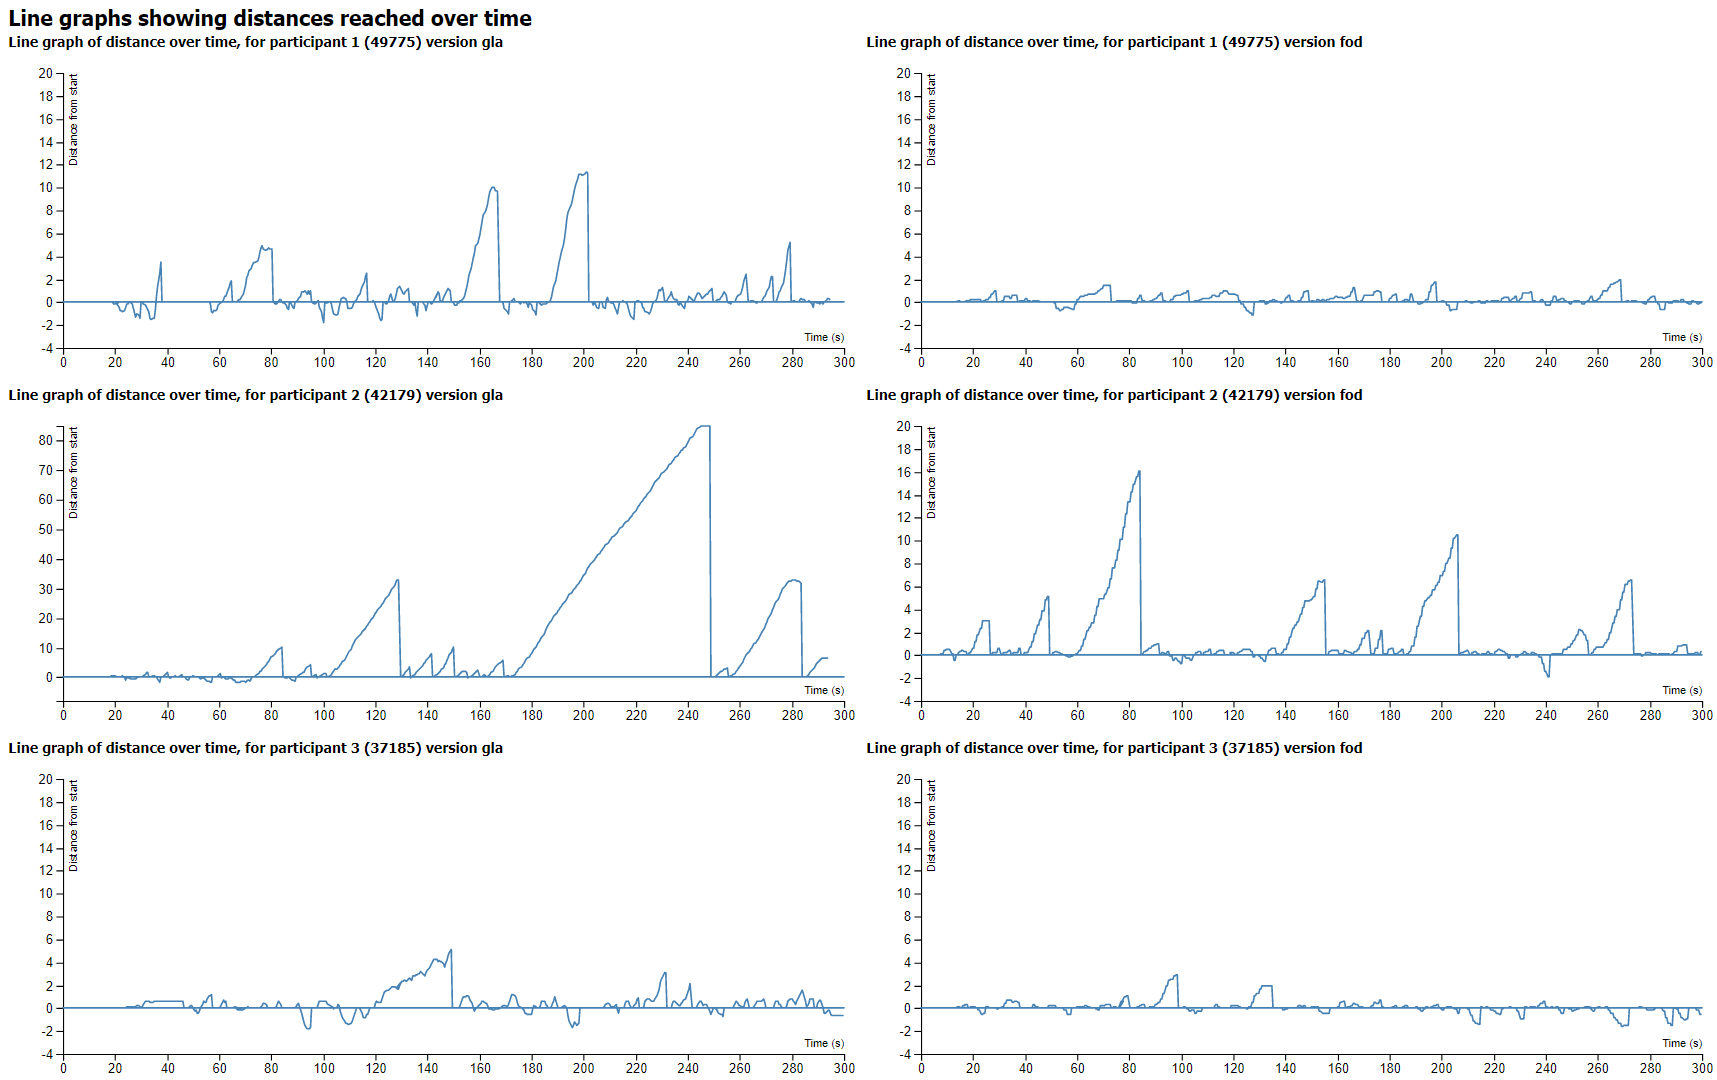
\includegraphics[scale=0.39]{assortedLineGraphs.PNG}}
% \caption{A selection of Distance over time graphs}
% \label{assorted}
% \end{figure}

\begin{figure*}[htb!]
    \centering
    \begin{subfigure}[t]{1\textwidth}
        \centering
        \includegraphics[height=2.2in]{line1a.pdf}
        % \caption{Line graph of distance over time, for participant 1 (49775) version fod}
        \label{line1}
    \end{subfigure}
    \begin{subfigure}[t]{1\textwidth}
        \centering
        \includegraphics[height=2.2in]{line2a.pdf}
        % \caption{Line graph of distance over time, for participant 2 (42179) version gla}
        \label{line2}
    \end{subfigure}
    \begin{subfigure}[t]{1\textwidth}
        \centering
        \includegraphics[height=2.2in]{line6.pdf}
        % \caption{Line graph of distance over time, for participant 2 (42179) version fod}
        \label{line3}
    \end{subfigure}
    \begin{subfigure}[t]{1\textwidth}
        \centering
        \includegraphics[height=2.2in]{line3a.pdf}
        % \caption{Line graph of distance over time, for participant 1 (49775) version gla}
        \label{line4}
    \end{subfigure}
    \caption{A selection of Distance over time graphs. Participant 1 playing version gla, fod, and repeated for Participant 2.}
    \label{assorted}
\end{figure*}


In this section, the controlled assessment will be explained, and the data recorded during the controlled experiment will be presented and analysed.

During the controlled experiment each participant was randomly placed into one of two groups.
The two groups played both versions of the game with instrumented code added. This allowed me to record the keys that the participants pressed, and the distance that they travelled over time. The implementation of the instrumented software is described in the Implementation chapter, Section \ref{studyimpl}.

% Each participant's usage of instrumented software is recorded.
Group A played my version (which I shall call version gla) first and then played the original (version fod, after its creator Bennet Foddy). Group B played them in the opposite order.
Each game was played for 5 minutes. When a participant moved on to a section of the user study where one of the games is played, a timer is started. When the 5 minutes is up, the page moves onto the next section. Between the two games there is a break page where the participant can press next when they are ready for the second version.
Participants have these 5 minutes to get as far as they can. Whenever they fall over they start again and can have as many restarts as they want in the 5 minutes. Figure \ref{assorted} shows examples of the distance some of the participants reached recorded over time.

\subsection{Restart Distances}
\label{restartDistances}

Figure \ref{assorted} shows some examples of the distance participants reached throughout the 5 minutes they played the version for. One can see the participants attempt to go forward, reach a distance, and then restart.
%Participant 2 reaches 85m at around 250 seconds.
To begin the analysis of this data I shall compare the distances that the participants reach at the end of each run; before they fall and restart, or run out of time. I will be calling these distances restart distances.

Figure \ref{glaRestarts} shows a histogram of all of these restart distances over the 30 participants for my JavaScript remake, version gla. Figure \ref{fodRestarts} shows the same but for the original QWOP, version fod.
These histograms contain all the restart distances for each version, and includes both participant groups.
The affect of the order a participant played the games is analysed later, as Section \ref{learningBias} investigates the learning bias of playing the other version first.

\begin{sidewaysfigure}[tbh]
    \begin{subfigure}[t]{1\textwidth}
    \centerline{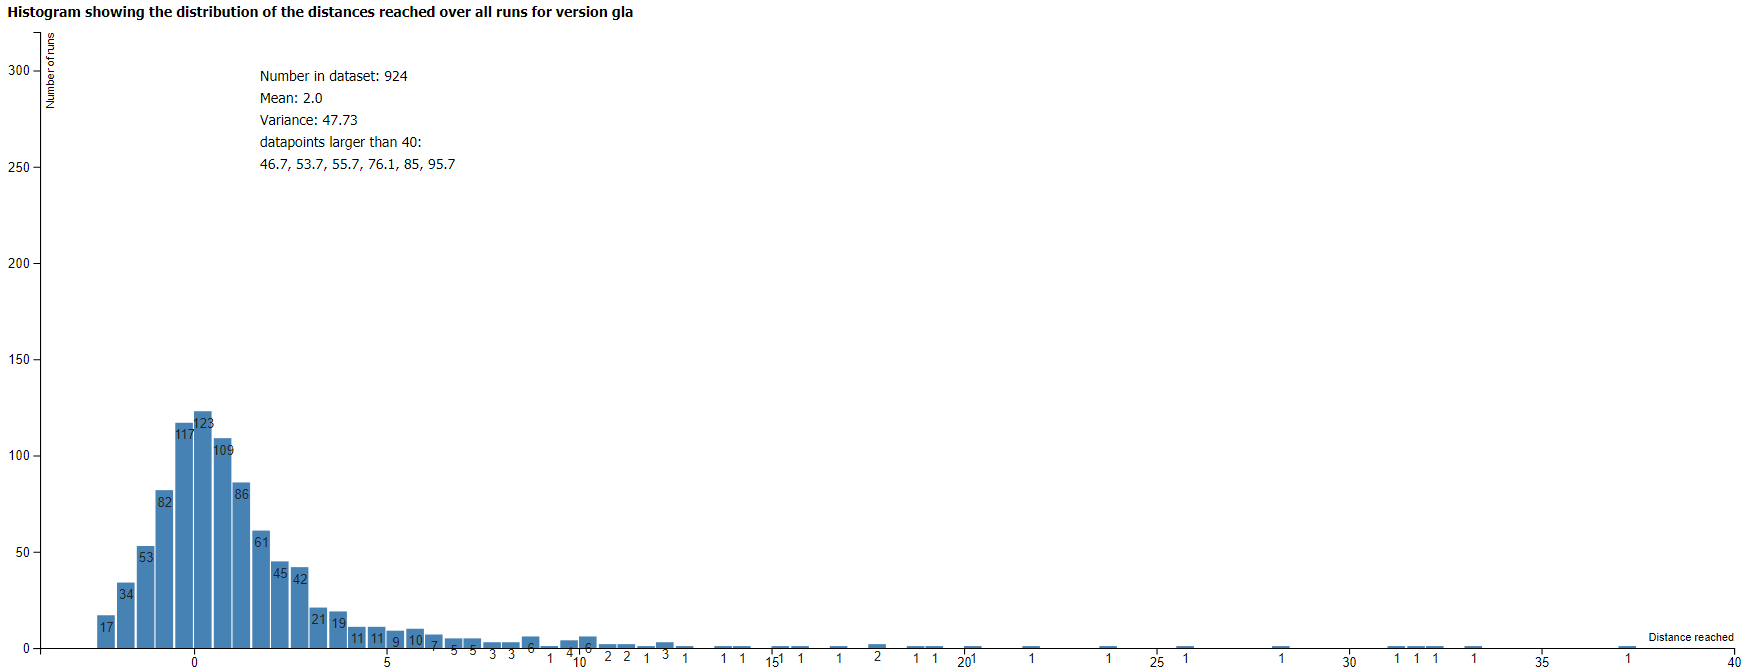
\includegraphics[scale=0.55]{glaRestarts.pdf}}
    \caption{Restart distances for version gla}
    \label{glaRestarts}
    \end{subfigure}

    \begin{subfigure}[t]{1\textwidth}
    \centerline{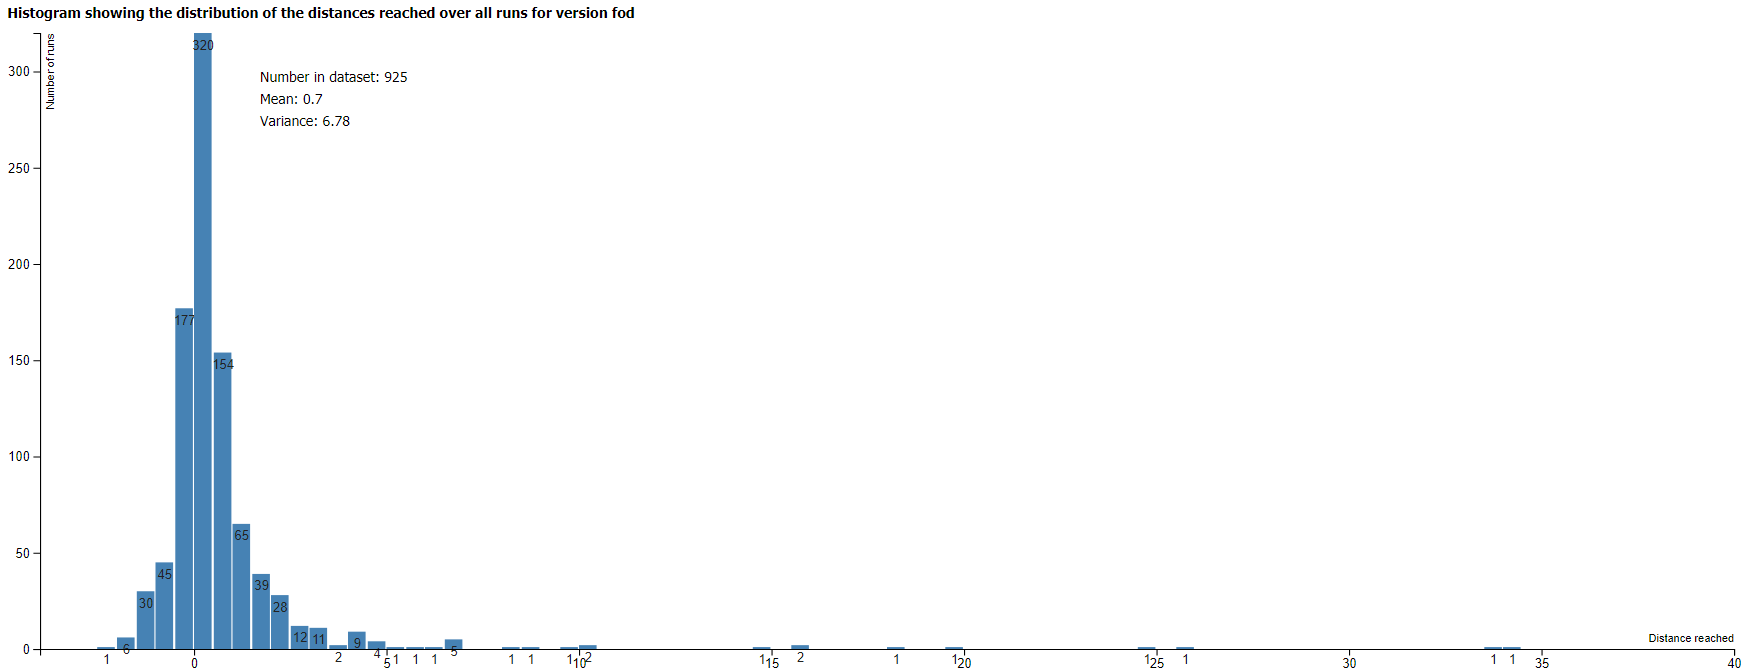
\includegraphics[scale=0.55]{fodRestarts.pdf}}
    \caption{Restart distances for version fod}
    \label{fodRestarts}
    \end{subfigure}
    
    \caption{A comparison of the distances participants reached over the two versions.}
\end{sidewaysfigure}

Figure \ref{glaRestarts} and \ref{fodRestarts} can be compared to see the change in the restart distances for the two versions. The graphs share a similar shape.
%, and also have a very similar area.
The total number of runs participants made when playing version gla is 924, and for version fod 925. This means that firstly, both graphs have almost exactly the same area, even though they look quite different. Secondly it shows that the average time a run lasted over all participants is very similar. My version is very faithful to the original in this regard, and this data is evidence that success criterion 2 -- having a similar gameplay experience -- is met.

%faithful to the original.
\begin{center}\begin{tabular}{ |p{3cm}|c| }\hline
Version& Average time of run (s)\\ \hline
gla & 9.74 \\ \hline
fod & 9.73 \\ \hline
\end{tabular}\end{center}

%It is striking that the total number of restarts is so close.
Another piece of evidence that supports criterion 2 is that both graphs have a similar shape. Both look like they belong to the Gaussian family of curves, although they are not symmetrical, as the athlete cannot go back further than the back wall.
The fact that participants fall backwards as often as they manage to go forward in both versions is a testament to the difficulty of controlling the athlete.
The curve for version gla in Figure \ref{glaRestarts} looks like a stretched version of the curve in Figure \ref{fodRestarts}. This shows that it was easier for participants to reach further in version gla.
This can be seen in the increase of the mean between the two versions, from 0.7 to 2.0, but more clearly in the increase of variance -- from 7 to 48 -- and in the maximum values the participants reached.

Even thought the track the athlete has to run down is 100 meters, the $x$-axis of the graph stretches until 40m so that the important section of the graph can be seen more clearly. No participant managed to go further than 40m for version fod, and the values above 40m for version gla are stated above the graph.

% The record distance the participants achieve changes for the different versions, and 
% todo: this makes it better


\subsection{Investigation of Learning Bias}
\label{learningBias}
%One thing you’ve not yet done in the Evaluation is see if there is a learning bias between the first and second versions the participants tried. For example, is it the case that those who used fod first, then did better at gla than those who did gla first? You should take advantage of your experimental design to test this.

When the participants started the user study, they were given a randomly generated participant ID. This number was used to link the questionnaire responses of each participant to the data logged during the controlled experiment. 
This number was also used to split the participants into the two groups for the A/B testing.
The benefit of using this random number to make the experiment a randomised control trial is that selection bias is minimised.

Another benefit of this experimental design is that the effect of playing one game before the other can be taken into consideration and not affect the analysis.

Figures \ref{glaBias} and \ref{fodBias} illustrate this learning bias affecting the participants.
For example in \ref{glaBias}, the learning bias for version gla can be seen.
The blue and khaki histograms both show the restart distances for the participants when playing version gla, however the blue histogram shows the restart distances for the participants in group A and the khaki for participants in group B.

\begin{sidewaysfigure}[tbh]
% \centerline{\includegraphics[scale=0.39]{learningBiasAffectingGla.PNG}}
\centerline{\includegraphics[scale=0.6]{biasGla.pdf}}
\caption{Learning bias affecting version gla}
\label{glaBias}
\end{sidewaysfigure}

The participants in group A play version gla first, whereas the participants in group B play version fod first, and so group B have the advantage of playing version fod beforehand.
This learning bias can be seen in Figure \ref{glaBias} to have a small effect on the performance of participants playing version gla. There is a small increase of the number of attempts from 427 to 497, and these are mostly manifested between 0 and -1, otherwise the curves are very similar.
% todo KS if time
This seems likely down to chance as there would be no reason for preceding play time of version fod to cause participants to fall over backwards more often.
%perhaps participants who had experienced version fod being more tricky to control, had already resorted to less methodical strategies.

\begin{sidewaysfigure}[tbh]
% \centerline{\includegraphics[scale=0.39]{learningBiasAffectingFod.PNG}}
\centerline{\includegraphics[scale=0.6]{biasFod.pdf}}
\caption{Learning bias affecting version fod}
\label{fodBias}
\end{sidewaysfigure}

Figure \ref{fodBias} takes the same approach but for version fod. Group B played version fod first, and group A played fod after playing version gla. Again the layered histograms visualise the effect that playing the other version beforehand has, showing the group with the learning bias in Khaki.
This time there is a different effect. Learning from version gla reduced the number of attempts made by 15 participants from 530 to 395.

% todo: finish




\section{Second Questionnaire}
\label{q2}

Participants complete the second questionnaire after they have played both versions of the game. It contains questions aimed at comparing the two versions. The questions and the answers participants could pick from are available in Appendix \ref{qs2}.
This part of the evaluation analyses the participants views of the different versions.

Figure \ref{successfull} shows the results for the question ``Which version of the game do you think you were more successful at?''. 
\begin{figure}[tbh]
    \begin{center}
    \begin{tabular}{ |p{6cm}|c|c|c| }
      \hline
    Version& \multicolumn{3}{|c|}{Frequency of response} \\ \cline{2-4}
    & Group A& Group B&Total\\ \hline\hline
    First played   & 8 & 5  & 13 \\ \hline
    Second played  & 7 & 10 & 17 \\ \hline\hline
    Version gla    & 8 & 10 & 18 \\ \hline
    Version fod    & 7 & 5  & 12 \\ \hline
    \end{tabular}
    \end{center}
    \caption{Participant opinion of whether they were more successful at the first or second version.}
    \label{successfull}
\end{figure}
%could look at thought vs reality but doesn't seem that useful?
For this question the answers the participants had to choose from were ``The first version'' and ``The second version''. This removes bias towards either version compared with giving the participants a choice between the two versions identified by their differences.
The different participant groups played the games in a different order, so \ref{opinions} shows the results that the participants gave, and how they translate into which version participants thought they were more successful at overall.

% Here are the questions, with the figures containing the data.
Figure \ref{opinions} contains the data of the responses to the question ``Which version felt like you had more control over the athlete?'' and `` Which version did you enjoy more?''
\begin{figure}[tbh]
    \begin{center}
    \begin{tabular}{ m{4cm}|c|c|c|c||c|c||c|c| }
    \cline{2-9}
     & \multicolumn{2}{|c|}{Group A} & \multicolumn{2}{|c|}{Group B} & \multicolumn{4}{|c|}{Total over groups} \\
    \cline{2-9}
    &First &Second &First &Second &&&& \\
    &version &version &version &version &gla&fod&First&Second \\
    &(gla)&(fod)&(fod)&(gla)&&&& \\ \hline
    \multicolumn{1}{ |m{4cm}| }{Which version felt like you had more control over the athlete?}& 7 & 8 & 4 & 11 & 18 & 12 & 11 & 19 \\ \hline
    \multicolumn{1}{ |m{4cm}| }{Which version did you enjoy more?}   & 9 & 6 & 5 & 10 & 19 & 11 & 14 & 16  \\ \hline
    \end{tabular}
    \end{center}
    \caption{Results of participant choice of version}
    \label{opinions}
\end{figure} 
Similar to the question above, both of these questions gave the choice between the first and second version. Taking into account the different participant groups, 19 of the 30 participants said they found version gla to be more enjoyable than version fod. This is strong evidence for the third success criterion:

\begin{displayquote}
    ``My version aims to be more playable for a typical player and I will quantify the improvement in a user study.''
\end{displayquote}


Figure \ref{firstHelpedSecond} gives the responses to the question ``Do you think playing the first version of the game improved your performance in the second version?''
\begin{figure}[tbh]
    \begin{center}
    \begin{tabular}{ |p{6cm}|c|c|c| }
      \hline
    Opinion whether playing the first& \multicolumn{3}{|c|}{Frequency of response} \\ \cline{2-4}
    helped improve the second& Group A& Group B&Total\\ \hline
    Definitely     & 1 & 5 & 6 \\ \hline
    Maybe          & 5 & 7 & 12\\ \hline
    I'm not sure   & 3 & 0 & 3 \\ \hline
    Maybe not      & 3 & 0 & 3 \\ \hline
    Definitely not & 3 & 3 & 6 \\ \hline
    \end{tabular}
    \end{center}
    \caption{Participant opinion of whether playing the first game helped improve their score for the second, by group.}
    \label{firstHelpedSecond}
\end{figure}
%This in relation to the bias section earlier

% say about answers to choose from and why good from
% https://www.tech.cam.ac.uk/Ethics_guidance/Survey-Methods

% open coding?








%%%%%%%%%%%%%%%%%%%%%%%%%%%%%%%%%%%%%%%%%%%%%%%%%%%%%%%%%%%%%%%%%%%%
%%%%%%%%%%%%%%%%%%%%%%%%%%%%%%%%%%%%%%%%%%%%%%%%%%%%%%%%%%%%%%%%%%%%
%%%%%%%%%%%%%%%%%%%%%%%%%%%%%%%%%%%%%%%%%%%%%%%%%%%%%%%%%%%%%%%%%%%%
%%%%%%%%%%%%%%%%%%%%%%%%%%%%%%%%%%%%%%%%%%%%%%%%%%%%%%%%%%%%%%%%%%%%
%%%%%%%%%%%%%%%%%%%%%%%%%%%%%%%%%%%%%%%%%%%%%%%%%%%%%%%%%%%%%%%%%%%%
%%%%%%%%%%%%%%%%%%%%%%%%%%%%%%%%%%%%%%%%%%%%%%%%%%%%%%%%%%%%%%%%%%%%
%k Conclusion (eval+conc ~ 2500)
\chapter{Conclusion}

My project is a success. I developed my own version of QWOP in JavaScript,
built a software system to evaluate my version, instrumented my version and the original QWOP, and run a controlled experiment to compare the versions.

The user study made use of A/B testing to let me control for ordering effects.
I have used survey methods to perform both quantitative and qualitative assessment of user perceptions of my software, which has shown that my version improves the experience for most players.
The data from the study has shown that I have met the success criteria. Firstly my version is faithful to the original. players have a similar experience, as the average time for a run is almost identical, and the distribution of distances that participants reach has the same pattern for each version.
Secondly my version is more playable for the typical player. The user study has shown that players could reach further down the track, and 19 of the 30 participants enjoyed my version more.

%as they could reach further, and felt that they had more control over the athlete.

In regards to the language choice, JavaScript was very well suited to the task because of the availability of Phaser and the ease of integrating with the evaluation system.
The mature debugging support of Chrome also helped 
Using a dynamically typed language did not create any problems, and as the scope of the project was not a large size, it was clearly a good choice.

%spiral method agile lectures chat?

%Phaser p

%In retrospect it
% Good in some respects
\appendix


\chapter{Project Proposal}

%r% Note: this file can be compiled on its own, but is also included by
% diss.tex (using the docmute.sty package to ignore the preamble)
\documentclass[12pt,a4paper,twoside]{article}
\usepackage[pdfborder={0 0 0}]{hyperref}
\usepackage[margin=25mm]{geometry}
\usepackage{graphicx}
\usepackage{parskip}
\hypersetup{
    colorlinks=false,
    linkcolor=blue,
    filecolor=magenta,      
    urlcolor=blue,
}
\begin{document}

\begin{center}
\Large
Computer Science Tripos -- Part II -- Project Proposal\\[4mm]
\LARGE
QWOP in JavaScript \\[4mm]

\large
George Andersen, gla23, Robinson College

\today

\end{center}

\vspace{5mm}

\textbf{Project Supervisor:} Dr A.~Beresford

\textbf{Director of Studies:} Prof A.~Mycroft

\textbf{Project Overseers:} Prof R.~Anderson \& Prof J.~Bacon

% Main document

\section*{Introduction}

% QWOP Description
QWOP is a 2008 ragdoll-based browser video game created by Bennett Foddy. Players control an athlete using only the Q, W, O, and P keys. The aim of the game is to complete a 100m race without falling over, which is a lot harder than it first seems.
Once the athlete reaches the end of the 100m, the player is given the time taken to complete the race. If a player can complete the 100m they can then try to do it as quickly as possible. After the game went viral in 2010, people have been trying to break the world record, one speed-run video attempting this on YouTube has 2.5 million views.
%The game helped Foddy's site reach 30 million hits.

QWOP uses a ragdoll physics simulation for the athlete. Each part of the runner's body is a rigid body with its own velocity, rotation and other physical quantities. It has joint constraints with connecting rigid bodies which allows the body to move without ending up in improbable or impossible positions.
The simulation also emulates muscles that can be controlled with the Q, W, O and P keys, so that the user can make the runner move. 
Whilst the Q key is held down, the runner's right thigh is driven forward and his left thigh is driven backward, and the W key does the opposite. The O and P keys do the same but for the calves.
Though the objective of QWOP is simple, it has been notorious for being difficult to master due to its controls with the Q, W, O and P keys.

 %Look up the correct terminology for this kind of system. Clearly you need to model some of the physics, but you perhaps also need to look up "forward kinematics", "inverse kinematics" and similar. An hour or two on Wikipedia now will help you work out the basics and how to describe your approach more precisely.

% Outline of plans (remake using JS + Phaser)
In this project I will make a new build of QWOP in JavaScript using Phaser. Phaser has a physics system called P2 that can be used to recreate the physics behind QWOP.

Phaser has objects called \emph{sprites} which can be used to create the game. Each of these can be attached to a P2 physics body used in Phaser's P2 physics system. I can then build on this system to give these bodies the correct physical properties.
More details on how this will work can be found in the Work to be done section.


%After making the physics simulation I would need to add graphics to the joints to make it look as well as run like a human. Another thing that would need to be added is a system to collision check when the man falls over, and measure how far the player got from the start. Then have it show your score and keep high scores etc just like in the real qwop.
% Deterministic scoring, based on your later comments, sounds like something thing you would want to support.
 

\section*{Starting point}

%\emph{Describe existing state of the art, previous work in this area, libraries and databases to be used. Describe the state of any existing codebase that is to be built on.}

One major codebase the project will be using is Phaser, a JavaScript library designed to make games.
So far I have downloaded Phaser and used some of the examples to explore the physics engine.

I have also spent time familiarising myself with the tools I will be using for the project and working out a work flow. These include Git, GitHub, WampServer, Phaser and Sublime text with LaTeXTools.

\section*{Resources required}

%\emph{A note of the resources required and confirmation of access.}

For this project I shall use my own laptop running Windows.
My Laptop's specifications:
Intel i7 16GB RAM, 1 TB+8 GB SSHD, AMD R9 GPU.

If my laptop fails I can continue development on the MCS machines in the Computer Lab.

I will backup my code and the writeup on a private repository on GitHub.

I require no other special resources.

\section*{Work to be done}

%\emph{Describe the technical work.}

The project breaks down into the following sub-projects:

Each of these sections include researching how the task can be completed in the Phaser physics engine, and then creating it in the project.


 


\newcommand{\WorkA}{Create a ragdoll model of the runner's body out of Phaser sprites with correct distance constraints between sections so that it keeps together whilst collapsing to the floor. }
\newcommand{\WorkB}{Ensure the body has inertia, give the floor friction and apply other physics features so the body acts like a runner rather than collapsing on itself. }
\newcommand{\WorkC}{Make the athlete controllable using the Q, W, O and P keys. Receive this input into the game, and give the correct rotational force to each section of the body as in the original game. }
\newcommand{\WorkD}{Add constraints on how far a joint can rotate. Add these constraints on the model of the athlete so the runner has human-like joint constraints. }
\newcommand{\WorkE}{Add graphics to the body; render an image for each sprite joint in order that together they look like an athlete's body. }
\newcommand{\WorkF}{Calculate and display the distance the runner has moved from the start and how long it has taken. }
\newcommand{\WorkG}{Add collision detection with the floor for the parts of the body that touch the floor when the runner falls over. Restart the game when the athlete falls over. }
\newcommand{\WorkH}{Check whether the runner has finished the race by checking whether the distance travelled is over 100m, and if so, record the time it took to complete the race. }

\begin{enumerate}
\item \WorkA
\item \WorkB
\item \WorkC
\item \WorkD
\item \WorkE
\item \WorkF
\item \WorkG
\item \WorkH
\end{enumerate}


\section*{Success criteria}

%\emph{Describe what you expect to be able to demonstrate at the end of the project and how you are going to evaluate your achievement.}

At the end of the project I expect to be able to demonstrate a game similar to that of the original QWOP.
The athlete should have the same physical qualities that make it seem human, and the game should have the same gameplay items that make it work. The Work to be done section breaks down how this will be done in more detail.

I propose to test how successful the project is with a user study. Since the quality of a game is subjective, it is appropriate to do a user study to evaluate the project.

%you'll have to give some thought to the design of this study in order to ensure that it has ecological validity.
I will design the study to evaluate the project, giving some thought to ensure that it has ecological validity.
In the study I would aim to gain some quantitative data.
%then explain why a user study is the appropriate way of determining whether you've done well enough.
For example after playing each version for 10 minutes, what was the average distance travelled over these runs for each participant? How much time did each run take? Did the scores of each participant increase over time, and how could these changes be modelled for each version?
I would also collect some qualitative data via a questionnaire to discover which game they found most enjoyable, which they thought they did better on, which game felt more responsive to their input, and other comments.

Even though I am not aiming to replicate the behaviour of the original QWOP exactly, another evaluation metric I could use is does the athlete respond in similar ways in both versions to the same inputs? This could be checked by programming the same input into both the original and my version, and checking the athlete goes through the same type of movement. 
%As the original QWOP isn't deterministic, and I plan for my version to be, the movement is unlikely to match exactly. This test however would still be useful, as can check the movements are similar.
Since I will not have access to the internal workings of the original QWOP game, and therefore cannot code the input directly, I could use an AutoHotkey script to give the desired input consistently.



\section*{Possible extensions}

%{\em Potential further envisaged evaluation metrics or extensions.} add deterministic here

If I achieve my main result and still have spare time I shall try an experiment of creating an AI module that attempts to play QWOP. It could be broken down into these sections:

\begin{enumerate}
\item Design an encoding scheme (or multiple to see which works best) that can be used to control input to the game. Each instantiated value of the scheme (runner) can be used to control the input to a game. A deterministic version of the game will give the same score each time the same runner plays a game.

\item Provide the AI module with access to the rotations of the different joints whilst the athlete is running so that the AI can use this information.

\item Test runners giving them a fitness score of how far they managed to run before falling over.
  
\item Make a genetic algorithm that can repeatedly test runners, and mutate them with the effect of increasing the fitness of the runners over time.
\end{enumerate}

 
% Old version of explanation
%An extension goal is to make an ai module that would give input to the game with the aim of getting to the end of the race as fast as possible. It would take an output from the game of the rotations of the joints and other data needed to make the ai work, and would then give an input to the game that should be intelligent enough to run the 100m.

Previous work includes \href{https://dl.acm.org/citation.cfm?id=2598248}{this paper} \cite{ray2014evolving} that has been written about evolving QWOP gaits.
The writer tests various genetic algorithms to evolve a gait (walking motion) for the original QWOP.
To do this he uses a similar approach to the one I have described above. The difference is that since he is using the original game, there is no access to the internal workings of the game, and therefore he can only get information from the game using a screen capture.
He uses this to work out the current score, and this is the only information he uses to evolve the runners. Since I am making my own version, I have access to the data in the game, and so I could use this information directly.

I could try reimplementing some of the coding schemes or genetic algorithms the above paper uses, but I will have more options as I have the extra data to use.

The paper found that it was hard to input into the original QWOP so that it acted deterministically.
This made it harder for the genetic algorithms to be effective as one input to the game could give different scores on different tries.
%The problem was that when it would pick the runners as they got a higher score, this could be because they happened to get a higher score that time, rather than being an inherently better runner.
For this reason I shall make it an extension aim for my version to be deterministic.

% Make deterministic an extension
%Another thing that will make the project a success is that the game is deterministic; gives the same score each time a certain key combination is entered. I want to support this as it will be helpful for an extension idea that is explained in the possible extensions.
%To test this I can code an input into the game that can be repeated, rather than use input from the keyboard. If the game is deterministic, it will give the same score each time. A different method I could use is to make an AutoHotkey script that gives an input, and it can be run multiple times to check the score is the same each time.

%Another possible extension is making another model that isn't a human. %suggested by alan

\section*{Timetable}
%\emph {A workplan of perhaps ten or so two-week work-packages, as well as milestones to be achieved along the way. Provide a target date for each milestone.}

%Planned starting date is \today.

% You need to put down what you will do for each fortnight between the start of the project and the hand-in date. Please list specific dates. You should schedule a week off for Christmas. As a rule of thumb, you need to schedule some time for research in October; have the core up and running in January so that you can present it working at the overseer review; perform the evaluation in February and early March, perhaps intermixed with revisions and improvements. Schedule two weeks in early March for "contingency time / extensions"; the rest of the time should be left for write-up.


\begin{enumerate}
%Michaelmas weeks 3 and 4: 
\item \textbf{19th October-1st November} After handing in project proposal, I can start researching how exactly to get the physics engine to do what I want. 

%Michaelmas weeks 5 and 6:
\item \textbf{2nd - 15th November} Start implementation of the model of runner; \WorkA
\WorkB


%Michaelmas weeks 7 and 8: 
\item \textbf{16th - 30th November}
\WorkC
\WorkD

%Michaelmas vacation
\item \textbf{1st - 14th December}
Start of Michaelmas vacation: Go on student getaway with church, travel home, and visit my sister in Italy with parents.
\item \textbf{15th - 23rd December}
\WorkE
\WorkF
\item \textbf{24th - 28th December}
Time off for Christmas
\item \textbf{29th December - 8th January}
\WorkG
\WorkH
\item \textbf{9th - 14th January}
Go on Ciccu getaway before moving back to Cambridge for Lent term.

%Lent weeks 1 and 2: 
\item \textbf{15th - 31st January}
Finish off all the sections in work to be done so that I can present the core game working at the overseer review.
Write progress report so that it can be handed in before noon on the 2nd February.

%Lent weeks 3 and 4: 
\item \textbf{1st - 14th February}
Contingency time/extensions -- extra time here in case previous work sections take longer than expected. If work moves quicker than expected I can start to investigate making the AI or can start designing the user study.
Meet success criteria.


%Lent weeks 5 and 6:
\item \textbf{15th - 28th February}
Work on evaluating the project. Finish designing and perform the user study, and evaluate any extension work.
Give time for revisions and improvements of the project.

%Lent weeks 7 and 8:
\item \textbf{1st - 14th March}
Start writing dissertation main chapters.


%Easter vacation:
\item \textbf{15 March - 25th April}
Complete the dissertation first draft so that it can be handed in on the 23rd (the day before the first day of Easter full term) so that there is time to incorporate feedback.

%Easter weeks 1 and 2:
\item \textbf{26th April - 9th May}
Take into account feedback and work on enhancing draft and re-factoring into the final version.

%Easter term week 3:
\item \textbf{10th - 17th May}
Proof read dissertation and then give an early submission so as to concentrate on examination revision.

\end{enumerate}

\bibliographystyle{plain}
\bibliography{proposal} 

\end{document}


\chapter{Questionnaire questions}
\label{qs}

\section{First Questionnaire}
\label{qs1}
\begin{enumerate}
    \item What is your age?

    \item What is your gender?

    \item Have you played QWOP before, and if so, for how long do you think you have played in total?
      \begin{enumerate}
      \item Less than 10 minutes              
      \item Between 10 and 30 minutes         
      \item Longer than 30 minutes            
      \item A long time over multiple sessions
      \end{enumerate}
    \item On average how long do you spend playing some form of video games during a typical week outside term time?
      \begin{enumerate}
      \item Less than an hour     
      \item Between 1 and 5 hours 
      \item Between 5 and 20 hours
      \item More than 20 hours    
      \end{enumerate}
\end{enumerate}

\section{Second Questionnaire}
\label{qs2}
\begin{enumerate}
    \item Which version of the game do you think you were more successful at?
    \begin{enumerate}
      \item The first version.
      \item The second version.
    \end{enumerate}
    \item Which version felt like you had more control over the athlete?
    \begin{enumerate}
      \item The first version.
      \item The second version.
    \end{enumerate}
    \item Why do you think this was?

    \item Do you think playing the first version of the game improved your performance in the second version?
    \item Which version did you enjoy more?
    \begin{enumerate}
      \item The first version.
      \item The second version.
    \end{enumerate}
    \item Why do you think this was?
\end{enumerate}

\end{document}
